\begin{figure}[!ht]
    % \centering
    % \subfloat[Bayes]{
    %     \label{Bayes}
    %     \begin{tikzpicture}[scale=0.55, baseline]
    %     \begin{axis}[
    %         width=1.5 \linewidth,
    %         height=0.8 \linewidth,
    %         %media de tempo intruder
    %         ybar=3pt,
    %         %enlargelimits=0.10,
    %         legend style={at={(0.5,-0.15)}, anchor=north, legend columns=-1},
    %         ylabel=Tempo(s),
    %         xlabel=Threads,
    %         symbolic x coords={1, 2, 4, 8, 16, 32, 64, 128, 256, 512},
    %         xtick=data,
    %         ymin=0,
    %         ymax=30,
    %         bar width=7pt,
    %         % nodes near coords,
    %         nodes near coords align={vertical},
    %     ]
    %     \addplot+[error bars,y dir=both, y explicit] coordinates {
    %         (1,8.46)+-(1,0.12) (2,9.04)+-(2,2.15) (4,5.41)+-(4,2.01) (8,5.49)+-(8,2.70) (16,4.71)+-(16,2.14) (32,7.33)+-(32,5.74) (64,3.78)+-(64,1.99) (128,4.82)+-(128,1.20) (256,2.87)+-(256,0.84) (512,4.32)+-(512,1.69)
    %     };
    %     \addplot+[error bars,y dir=both, y explicit] coordinates {
    %         (1,8.86)+-(1,0.17) (2,7.02)+-(2,2.95) (4,5.52)+-(4,1.47) (8,6.03)+-(8,2.78) (16,5.75)+-(16,2.44) (32,5.92)+-(32,3.68) (64,4.36)+-(64,1.66) (128,4.78)+-(128,2.50) (256,3.78)+-(256,2.36) (512,5.34)+-(512,2.97)
    %     };
    %     \addplot+[error bars,y dir=both, y explicit] coordinates {
    %         (1,8.87)+-(1,0.14) (2,6.68)+-(2,1.10) (4,8.09)+-(4,5.99) (8,7.33)+-(8,3.29) (16,4.32)+-(16,2.09) (32,4.71)+-(32,0.94) (64,3.12)+-(64,1.09) (128,5.50)+-(128,1.87) (256,4.62)+-(256,2.12) (512,5.18)+-(512,1.52)
    %     };
    %     \addplot+[error bars,y dir=both, y explicit] coordinates {
    %         (1,8.80)+-(1,0.10) (2,6.87)+-(2,0.90) (4,14.29)+-(4,9.42) (8,4.60)+-(8,2.73) (16,5.56)+-(16,1.06) (32,3.95)+-(32,0.79) (64,8.22)+-(64,1.45) (128,9.40)+-(128,1.98) (256,3.48)+-(256,1.49) (512,8.61)+-(512,3.82)
    %     };
    %     \addplot+[error bars,y dir=both, y explicit] coordinates {
    %         (1,8.84)+-(1,0.21) (2,6.29)+-(2,2.84) (4,12.79)+-(4,5.91) (8,3.91)+-(8,1.84) (16,3.66)+-(16,1.03) (32,3.89)+-(32,0.97) (64,5.88)+-(64,3.19) (128,8.70)+-(128,3.51) (256,3.60)+-(256,1.96) (512,8.97)+-(512,5.75)
    %     };
    %     \legend {Tiny, Latency-Sequential, Latency-Chunks, Threshold-Sequential, Threshold-Chunks}
    %     \end{axis}
    %     \end{tikzpicture}
    % }
    
    \subfloat[Intruder]{
        \label{Intruder}
        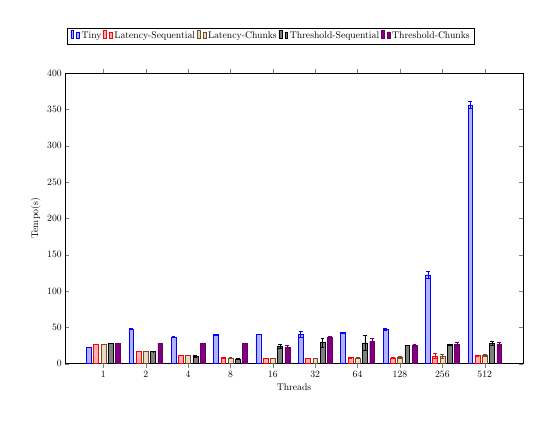
\begin{tikzpicture}[scale=0.35, baseline]
        \begin{axis}[
            width=1.5 \linewidth,
            height=1 \linewidth,
            %media de tempo intruder
            ybar=2.5pt,
            % enlargelimits=0.10,
            legend style={at={(0.45,1.1)}, anchor=south, legend columns=-1},
            ylabel=Tempo(s),
            xlabel=Threads,
            symbolic x coords={1, 2, 4, 8, 16, 32, 64, 128, 256, 512},
            xtick=data,
            ymin=0,
            ymax=400,
            bar width=5pt,
            % nodes near coords,
            nodes near coords align={vertical},
        ]
        \addplot+[error bars,y dir=both, y explicit] coordinates {
            (1,22.49)+-(1,0.11) (2,47.47)+-(2,0.69) (4,36.62)+-(4,0.59) (8,39.90)+-(8,0.89) (16,40.47)+-(16,0.35) (32,40.54)+-(32,3.55) (64,42.59)+-(64,0.29) (128,47.43)+-(128,1.97) (256,122.18)+-(256,4.64) (512,356.05)+-(512,5.11) 
        };
        \addplot+[error bars,y dir=both, y explicit] coordinates {
            (1,27.06)+-(1,0.18) (2,16.76)+-(2,0.13) (4,11.43)+-(4,0.10) (8,8.18)+-(8,0.13) (16,7.20)+-(16,0.06) (32,7.31)+-(32,0.14) (64,8.25)+-(64,0.81) (128,8.00)+-(128,0.37) (256,10.82)+-(256,3.29) (512,11.20)+-(512,0.86)
        };
        \addplot+[error bars,y dir=both, y explicit] coordinates {
            (1,26.90)+-(1,0.17) (2,16.89)+-(2,0.13) (4,11.50)+-(4,0.13) (8,8.10)+-(8,0.10) (16,7.21)+-(16,0.06) (32,7.28)+-(32,0.07) (64,7.61)+-(64,0.63) (128,9.11)+-(128,0.98) (256,10.40)+-(256,2.68) (512,11.59)+-(512,0.72)
        };
        \addplot+[error bars,y dir=both, y explicit] coordinates {
            (1,27.73)+-(1,0.05) (2,16.65)+-(2,0.16) (4,10.50)+-(4,1.10) (8,6.64)+-(8,0.23) (16,24.42)+-(16,2.56) (32,29.00)+-(32,6.41) (64,28.59)+-(64,10.33) (128,25.01)+-(128,0.29) (256,26.19)+-(256,1.25) (512,27.87)+-(512,2.82)
        };
        \addplot+[error bars,y dir=both, y explicit] coordinates {
            (1,27.96)+-(1,0.25) (2,28.12)+-(2,0.28) (4,28.11)+-(4,0.14) (8,28.17)+-(8,0.07) (16,23.01)+-(16,1.76) (32,36.20)+-(32,1.18) (64,30.24)+-(64,4.39) (128,24.97)+-(128,1.10) (256,26.99)+-(256,2.13) (512,27.18)+-(512,2.84)
        };
        \legend {Tiny, Latency-Sequential, Latency-Chunks, Threshold-Sequential, Threshold-Chunks}
        \end{axis}
        \end{tikzpicture}
    }
    \subfloat[Kmeans]{
        \label{Kmeans}
        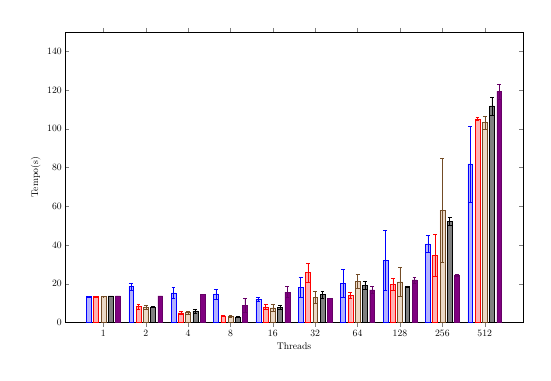
\begin{tikzpicture}[scale=0.35, baseline]
        \begin{axis}[
            width=1.5 \linewidth,
            height=1 \linewidth,
            %media de tempo intruder
            ybar=2.5pt,
            %enlargelimits=0.10,
            % legend style={at={(0.5,-0.15)}, anchor=north, legend columns=-1},
            ylabel=Tempo(s),
            xlabel=Threads,
            symbolic x coords={1, 2, 4, 8, 16, 32, 64, 128, 256, 512},
            xtick=data,
            ymin=0,
            ymax=150,
            bar width=5pt,
            % nodes near coords,
            nodes near coords align={vertical},
        ]
        \addplot+[error bars,y dir=both, y explicit] coordinates {
            (1,13.32)+-(1,0.05) (2,18.64)+-(2,1.86) (4,15.33)+-(4,2.68) (8,14.72)+-(8,2.44) (16,12.06)+-(16,0.95) (32,18.24)+-(32,5.19) (64,20.20)+-(64,7.21) (128,32.16)+-(128,15.30) (256,40.54)+-(256,4.28) (512,81.86)+-(512,19.67) 
        };
        \addplot+[error bars,y dir=both, y explicit] coordinates {
            (1,13.36)+-(1,0.05) (2,8.25)+-(2,1.41) (4,5.05)+-(4,0.53) (8,3.49)+-(8,0.45) (16,8.10)+-(16,1.15) (32,25.81)+-(32,4.77) (64,14.01)+-(64,1.61) (128,19.77)+-(128,3.11) (256,34.76)+-(256,10.90) (512,105.07)+-(512,0.66)
        };
        \addplot+[error bars,y dir=both, y explicit] coordinates {
            (1,13.39)+-(1,0.03) (2,8.05)+-(2,1.09) (4,5.13)+-(4,0.64) (8,3.37)+-(8,0.57) (16,7.62)+-(16,1.79) (32,13.01)+-(32,3.05) (64,21.35)+-(64,3.62) (128,21.05)+-(128,7.45) (256,57.98)+-(256,27.06) (512,103.22)+-(512,3.24)
        };
        \addplot+[error bars,y dir=both, y explicit] coordinates {
            (1,13.70)+-(1,0.00) (2,8.08)+-(2,0.39) (4,6.03)+-(4,1.01) (8,2.85)+-(8,0.20) (16,7.92)+-(16,1.01) (32,14.57)+-(32,1.81) (64,19.24)+-(64,2.21) (128,18.49)+-(128,0.48) (256,52.31)+-(256,2.27) (512,111.88)+-(512,4.66) 
        };
        \addplot+[error bars,y dir=both, y explicit] coordinates {
            (1,13.73)+-(1,0.00) (2,13.72)+-(2,0.00) (4,14.49)+-(4,0.02) (8,8.98)+-(8,3.78) (16,15.66)+-(16,2.82) (32,12.59)+-(32,0.01) (64,16.86)+-(64,1.83) (128,21.99)+-(128,1.45) (256,24.41)+-(256,0.44) (512,119.27)+-(512,3.89)
        };
        % \legend {Tiny, Latency-Sequential, Latency-Chunks, Threshold-Sequential, Threshold-Chunks}
        \end{axis}
        \end{tikzpicture}
    }
    
    % \caption{Tempo de execução (s) em NUMA variando o número de \emph{threads}.}
    % \label{temp}

\end{figure}
